In this section, we review the supporting runtime that is used by the compiler.
We focus mostly on the structure of the nodes since inference rules are compiled
from the point of view of the node data structure.

Figure~\ref{fig:node} presents the layout of the node data structures.  Each
node of the graph stores 4 main data structures: (1) the \emph{rule matching
   engine}; (2) a \emph{fact buffer} for storing incoming and temporary facts;
(3) the \emph{database of linear facts}; and (4) the \emph{database of
   persistent facts}.

\begin{wrapfigure}{r}{0.5\linewidth}
%\vspace{-1.2cm}
\begin{center}
   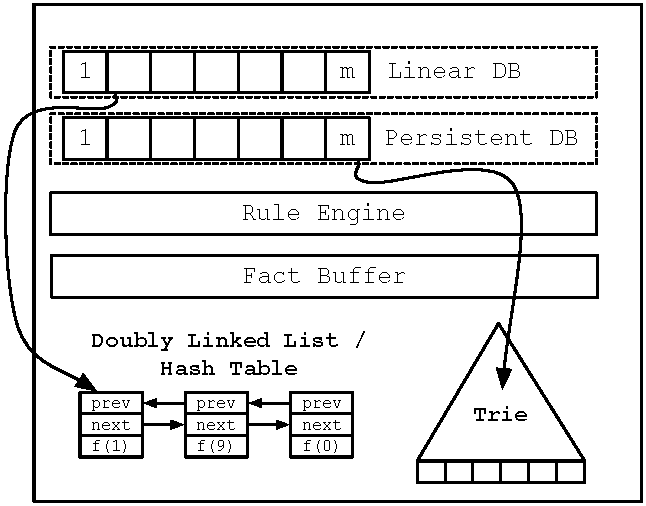
\includegraphics[width=1\linewidth]{figures/overview.pdf}
\end{center}
\caption{Node data structures.}
\label{fig:node}
%\vspace{-0.7cm}
\end{wrapfigure}


The rule engine maintains a simplified view of the two fact databases and
efficiently decides which rules need to be executed. For instance, if a rule $r$
needs facts \texttt{a} and \texttt{b} to be applied and the database already
contains \texttt{a} facts, once a \texttt{b} fact is derived, the rule engine
schedules $r$ to be executed. The compiler is responsible for the code that is
executed when a rule is scheduled.  A compiled rule contains instructions to
search and match facts from the database and to derive new facts when the body
of the rule is matched.

In this context, the organization of the database structures is critical because
linear facts can be retracted and asserted frequently. This means that the
database needs to allow fast insertions and deletions but also needs to have
reasonably fast mechanisms for lookup. The database of facts is partitioned by
predicate, therefore, each predicate can have its own data structure depending
on the patterns of access for that particular predicate. Linear facts are stored
using the following data structures:


\begin{itemize}

\item \emph{Doubly-Linked List Data Structures}. Each linear fact is a node of
   the linked list. Allows constant $\mathcal{O}(1)$ insertion and deletion of
   facts given the pointer of the target node. Although lookup operations take
   linear time, this is not critical since most predicates tend to have a small
   number of facts.

\item \emph{Hash Table Data Structures}. For predicates with many facts we use
   hash tables. Hash tables are efficient for repetitive lookup operations
   using a specific argument (i.e., searching for facts with a concrete value)
   and build upon lists by hashing facts using a specific argument and then
   using separate chaining with doubly-linked lists for collision resolution.
   Hash tables are, on average, $\mathcal{O}(1)$ for insertion, deletion and
   lookup, however they require more memory.

\end{itemize}

For persistent tuples, we use \emph{Trie Data Structures}, which are trees where
facts are indexed by a common prefix. Since persistent facts are never deleted,
it's not expensive to index facts by a common prefix, which also tends to save
memory in the long run.

